\subsubsection{Overview}
\label{sec:inst_overview}

The SmartRobotinoInstructionPlanner component is responsible for the task coordination between all between various components used in the software written for the 
Robocup Logistics League. This component was introduced by the 2016 team of Ulm University of Applied Science. The intention behind this component was that a master robot should process the information received from the Robocup Logistics Referee Box and start instructing the other Robotinos on the field. Different functionalities like driving around the field or detecting some MPS stations is implemented in various components but not in the SmartRobotinoInstructionPlanner component. For instructing these components a task sequencer (which is called SmartLispServer) is used and the task or logic blocks are written in a language called SmartTCL which is based on Common Lisp //todo cite to SmartTCL. \\ 

The SmartRobotinoInstructionPlanner is connected to the RefboxServer component using two SmartSoft ports. One port is for transmitting messages from the Referee Box to the Instruction Planner and the other is for sending information about detected MPS stations back to the Referee Box. For sending information between those two components, special communication objects are used which makes it easier to parse and process those messages. These messages are based on a special DSL for communication objects which are later converted to C++ classes. With these classes those messages can be easily processed within those components. //ref to SmartSoft Communication objects. \\

The first design of the Instruction Planner was developed on the fact that when the exploration phase starts, the Referee Box sends a list of possible zones for the exploration. In these possible zones, MPS stations for the team can be located. It was intended that a master robot should process this list of zones and splits this list up into three parts. These parts can be deployed on all Robotinos for exploring the field. This was the only intention of the SmartRobotinoInstructionPlanner, all other instruction logic should be implemented in the sequencer component. In 2017 the Robocup Logistics League committee removed these list of zones from the rules to make it harder for the teams to archive a successful exploration phase. Therefore the intentional implementation was now meaningless and therefore abandoned. So the meaning of the Instruction Planner was moved more the the instruction of various components of the Robotinos software. \\


\subsubsection{Previous implementation}
\label{sec:previous}

//maybe will be discarded

As described in (reference to book of knowledge) the Instruction Planner was designed for planning and coordination of other components on the master Robotino (the one who manages the connection between the Refbox and all Robotinos) but also all other robotinos. This means that it was designed that on all slave robotinos only the necessary parts like driving, detection or docking should run. All coordination should be done by the instruction planner on the master robotino. The intention behind this idea was that the referee box was sending a list of probable zone which can contain a MPS station for detection. This list of MPS stations was then split by an algorithm into three parts (one for each robot), so that a concurrent exploration and detection of the game field can be archived. In the 2017 scenario (link to 2017 rules) this feature was discarded from the competition. In the newer scenario there is no information whether there is a MPS station or not. Therefore this feature was also discarded in the new design for the 2017 competition \ref{sec:new_design}.  \\



\begin{figure}[h]
\centering
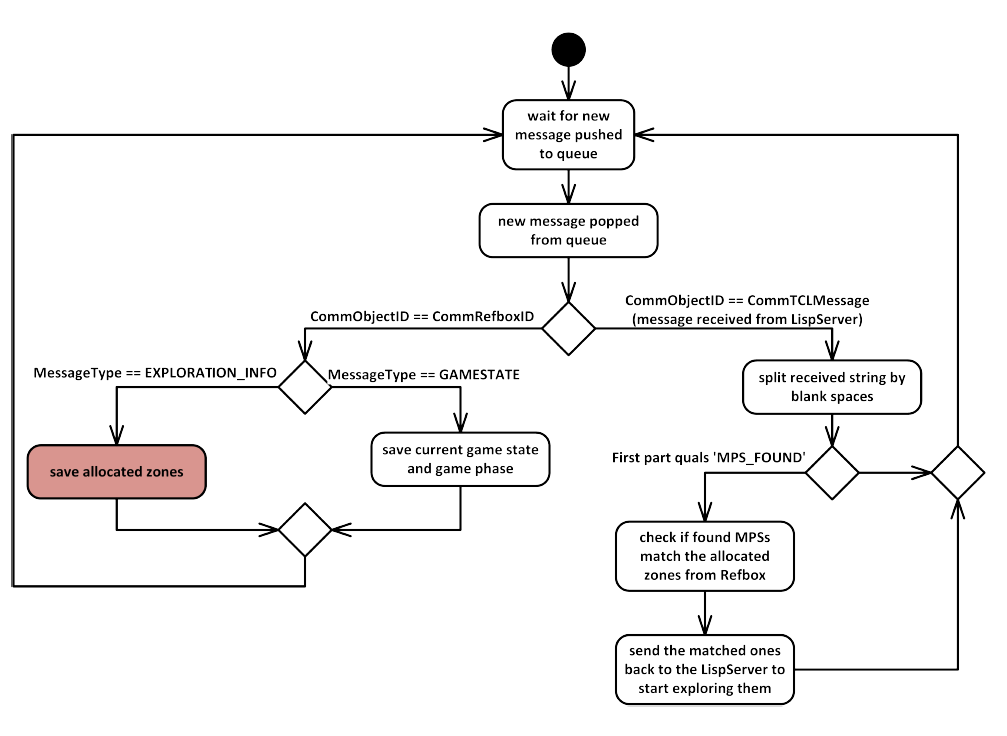
\includegraphics[scale=0.5]{pic/2016_flow_graph.png}
\caption{Flow of the instruction planner in the 2016 scenario}
\label{fig:ip2016}

\end{figure}


As it can be seen in figure \ref{fig:ip2016} the 2016 design of the Instruction Planner was not a full implementation of the exploration phase. In 2016 the team implemented some basic functionality which enables it to drive around the field and react on a gamestate. But nonetheless the team implemented the foundation of the robotino software which was then refined to implement a full version of the exploration phase in 2017. In Figure \ref{fig:ip2016} the control flow of the instruction as it was the state when the team took over the project can be seen. The first thing the Instruction Planner does is to wait for incoming messages. If a message was received it can usually be two types (either a message from the Referee Box or from one of the other components via the SmartLispServer). If the message was from the RefBoxServer it can be either a Exploration\_INFO message or a GAMESTATE message. In the 2017 implementation only the GAMESTATE message is used because the EXPLORATION\_INFO was discarded. \\

If the message was a CommTCLMessage (i.e. the message was sent by the SmartLispServer) only the MPS\_FOUND message was handled. The algorithm implemented by the 2016 team first checked if the found MPS stations matched some of the probable zones send by the Referee Box. If this was the case than the matched zones are send back to the LispServer for further exploration (i.e. approaching the MPS and start scanning of the AlvarTag). \\

The return of the detected MPS stations to the Referee Box was not implemented in the Instruction Planner but in the SmartAlvarTagDetection component. For this there was a connection established with an TagEventClient in the SmartRefBoxServer and a SmartEventServer in the AlvarTagDetection. Using this path the Instruction Planner hat no information about the behavior of the MPS station. Therefore in a future implementation of the production phase the Instruction Planner has no idea which station to approach when producing a element by a cap station or a ring station. This design was also revoked in the 2017 implementation where the AlvarTagDetection is now connected to the Instruction Planner and AlvarTag information will be handled there. 
  
 

\subsubsection{Revised design of the SmartRobotinoInstructionPlanner}
\label{sec:new_design}

As described in \ref{sec:inst_overview} the 2016 design of the Instruction Planner had a few flaws which made it not really adequate for the 2017 competition. Therefore the design was cleaned up and a revised version of the Instruction Planner was created. As described in section \ref{sec:previous} the behavior of the exploration phase was implemented in a lot of different components. To narrow this down it was decided that the Instruction Planner is now responsible for the main control of the all components. This means that the whole exploration phase is implemented in the Instruction Planner. All other components have only domain specific functionality, i.e. that the AlvarTagDetection is only responsible for tag detection and not for sending it back to the Referee Box. \\

The main message processing task is still implemented in the InstructionPlanerTask class. This means that in this class Refbox messages or CommTCLMessage objects can be received or transmitted. 


\begin{figure}[h]
\centering
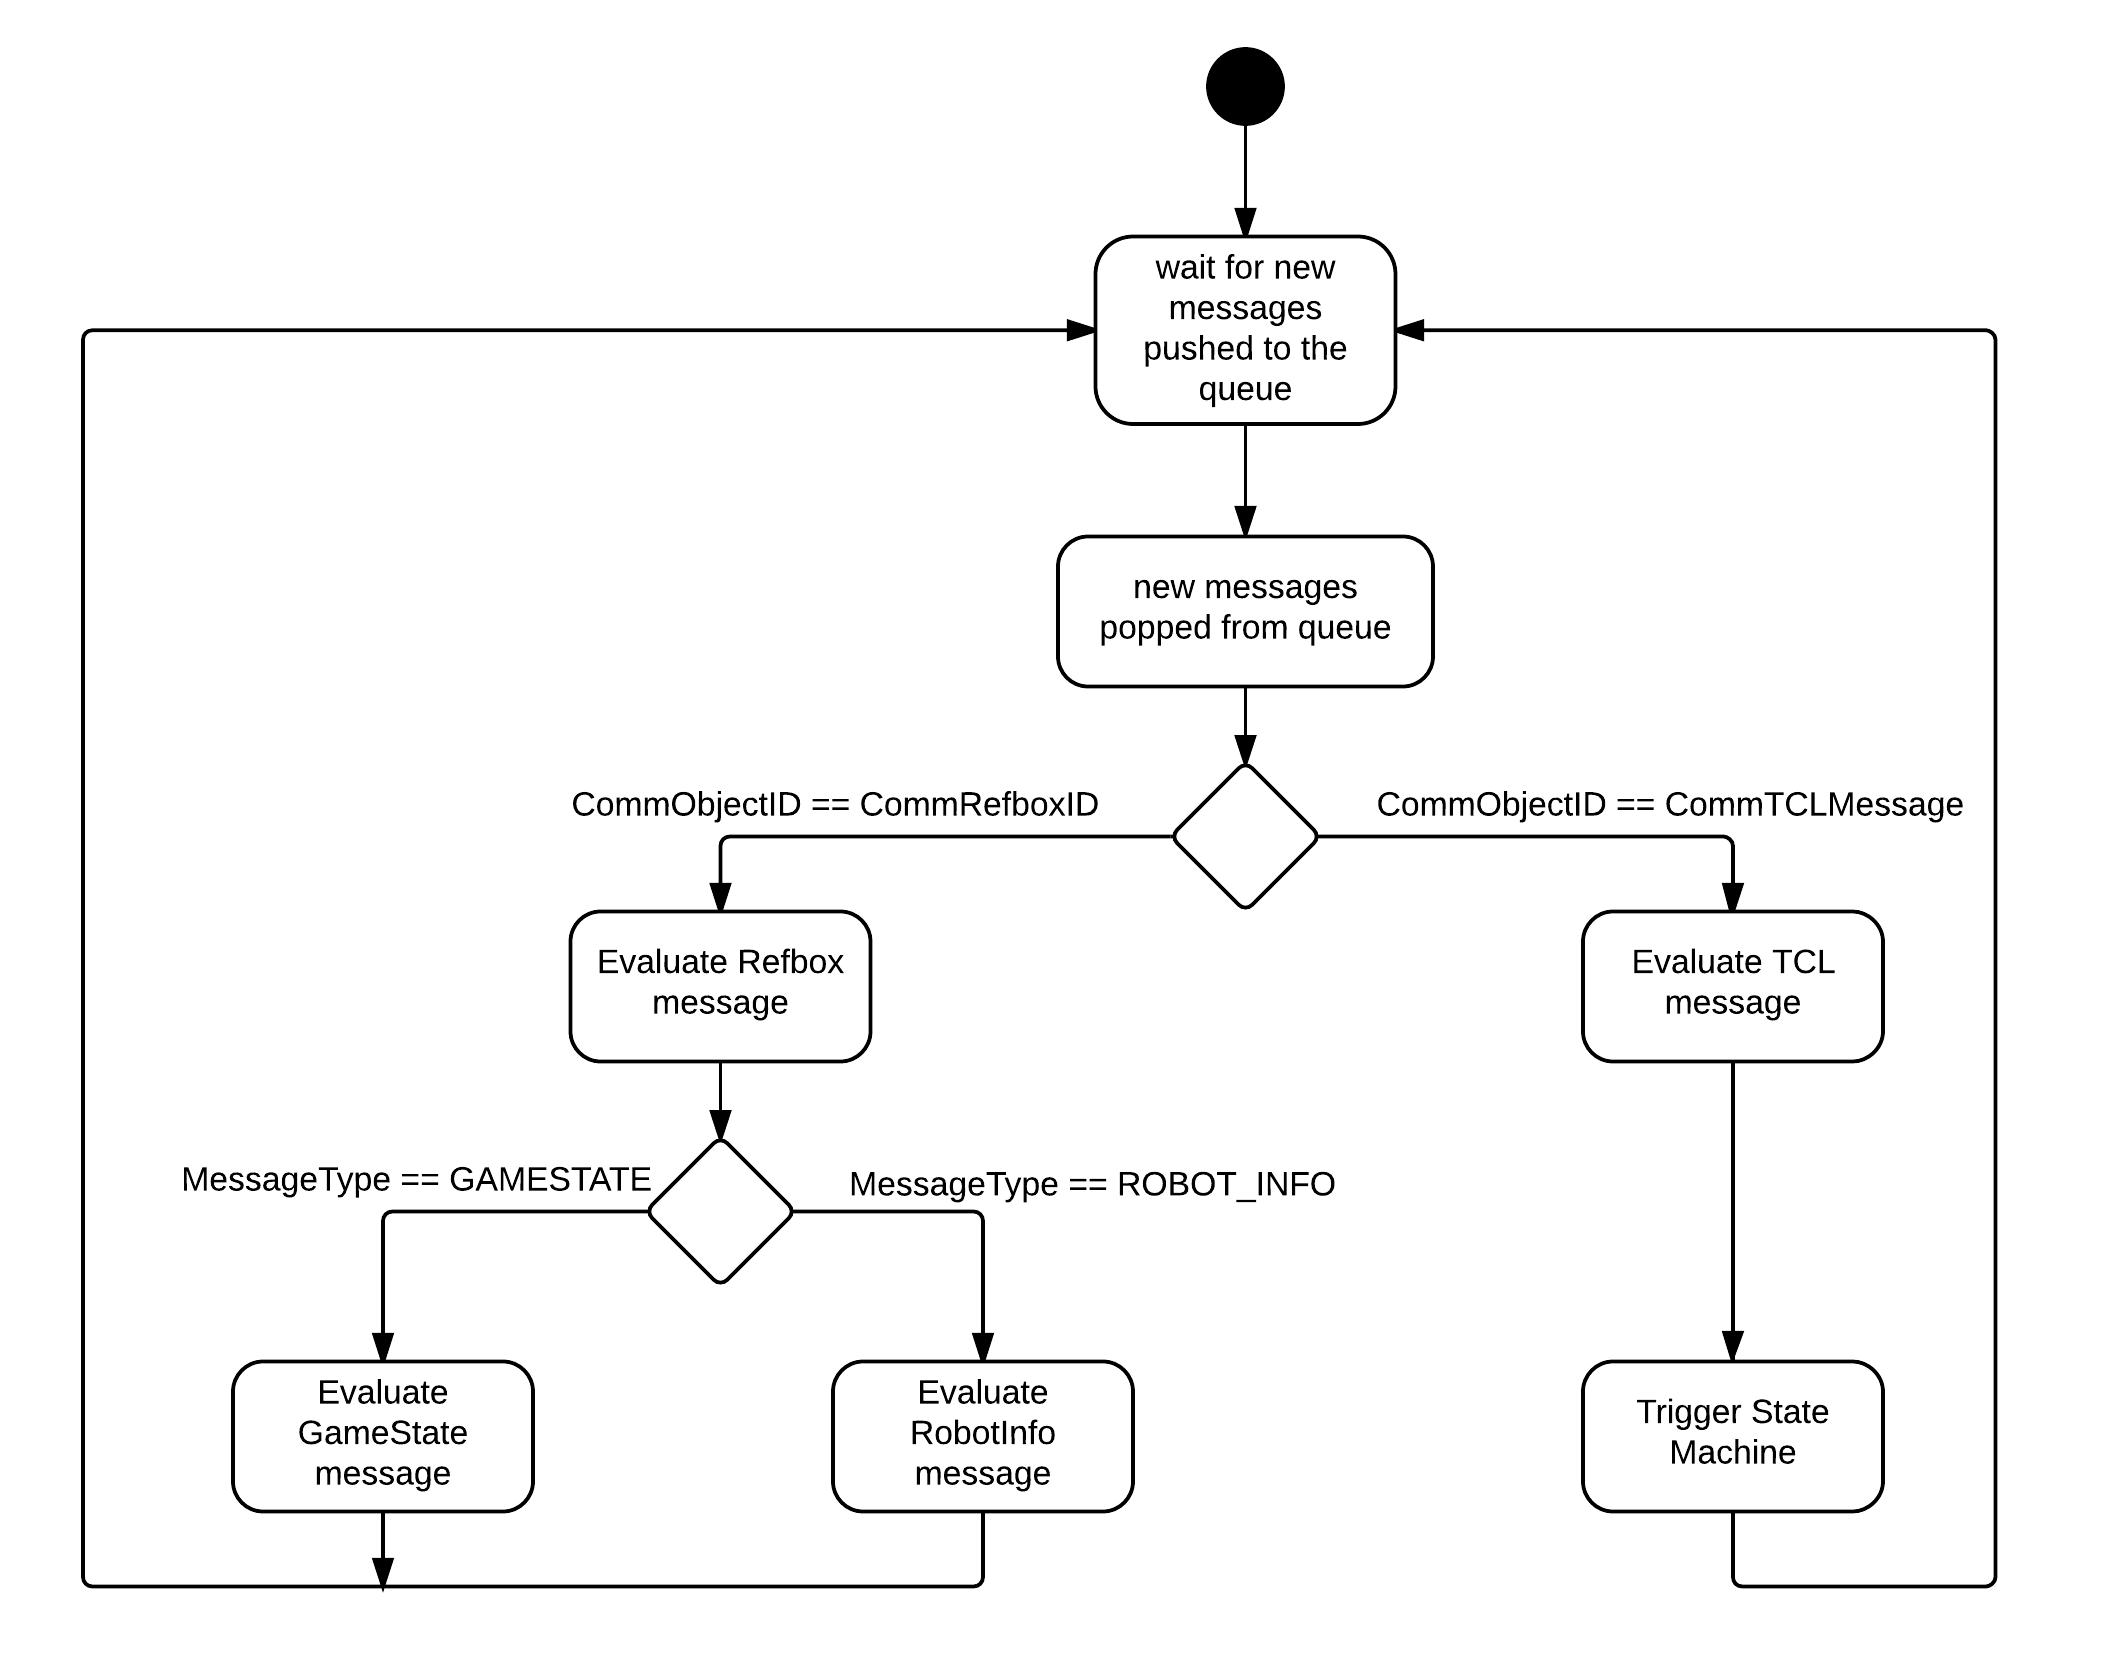
\includegraphics[scale=0.25]{pic/InstructionPlannerTask.png}
\caption{The control flow of the Instruction Planner Task}
\label{fig:instructionplannertask}
\end{figure}
 
As it can be seen in figure \ref{fig:instructionplannertask} the control flow of the InstructionPlannerTask is a little bit different than in 2016. If a new message is popped from the queue it is checked whether it is a CommRefBox- or a CommTCLMessage. In case of a CommRefBoxMessage it is checked either the gamestate is checked or the robot\_info. If the evaluation of either one of both is done the control flow jumps back to the start and waits for another incoming message. In case of a CommTCLMessage first the message header is evaluated and according to this information a event is triggered in the state machine which is implemented in the RobotState class. With this step the responsibility is handovered to the state machine and after this the control flow jumps the start and waits for another message. \\ 

Table \ref{tab:tcl_state} shows various TCL messages which are send from the components and the events which are then triggered in the state machine: \\

\begin {table}[h]
\caption{TCL messages and State machine events}
\label{tab:tcl_state}
\begin{center}

\begin{tabular}{|l|l|}
\hline 
TCLmessage & State machine event \\ 
\hline 
MPS\_FOUND & EV\_MPS\_FOUND \\ 
\hline 
NO\_MPS\_FOUND & EV\_MPS\_NO\_FOUND \\ 
\hline 
GOAL\_REACHED & EV\_GOAL\_REACHED\\ 
\hline 
ALVAR\_TAG & EV\_FOUND\_TAG \\ 
\hline 
MARKER\_NOT\_DETECTED & EV\_FOUND\_NO\_TAG \\ 
\hline 
ALVA\_TAG & EV\_FOUND\_TAG \\ 
\hline 
DOCKING\_DONE & EV\_DOCKING\_DONE \\ 
\hline 
DOCKING\_NO\_STATION & EV\_DOCKING\_NO\_STATION \\ 
\hline 
\end{tabular} 
\end{center}
\end {table}

\bigskip

By using this table the algorithm can make a lookup and checks which event should be triggered inside the state machine. This is a basic lookup algorithm and is the implementation of the "Evaluate TCL message" and "Trigger State Machine" path of figure \ref{fig:instructionplannertask}. The state machine which implements the exploration phase can be seen in section \ref{sec:state_machine}. 
  

\subsubsection{State machine}
\label{sec:state_machine}

Figure \ref{fig:statemachine} shows the statemachine for the exploration phase scenario. This statemachine was implemented inside a class called RobotState. When the robotino software boots up the first state which is entered is the initial state. In this state the robot does nothing except that it waits for a signal by the referee box which triggers the EV\_EXPLORATION event. Using this event the robot knows that the exploration phase has begun and the robot can make a transition into detection state. In the detection state the robot drives around the field and tries to detect MPS stations. The detection will be done by the MPSDocking component. If this component has found a station on the field it reports this back via the LispServer component to the Instruction Planner. If a one or more MPS stations were found the State machine makes a transition to the Approaching state. \\


\begin{figure}
\centering
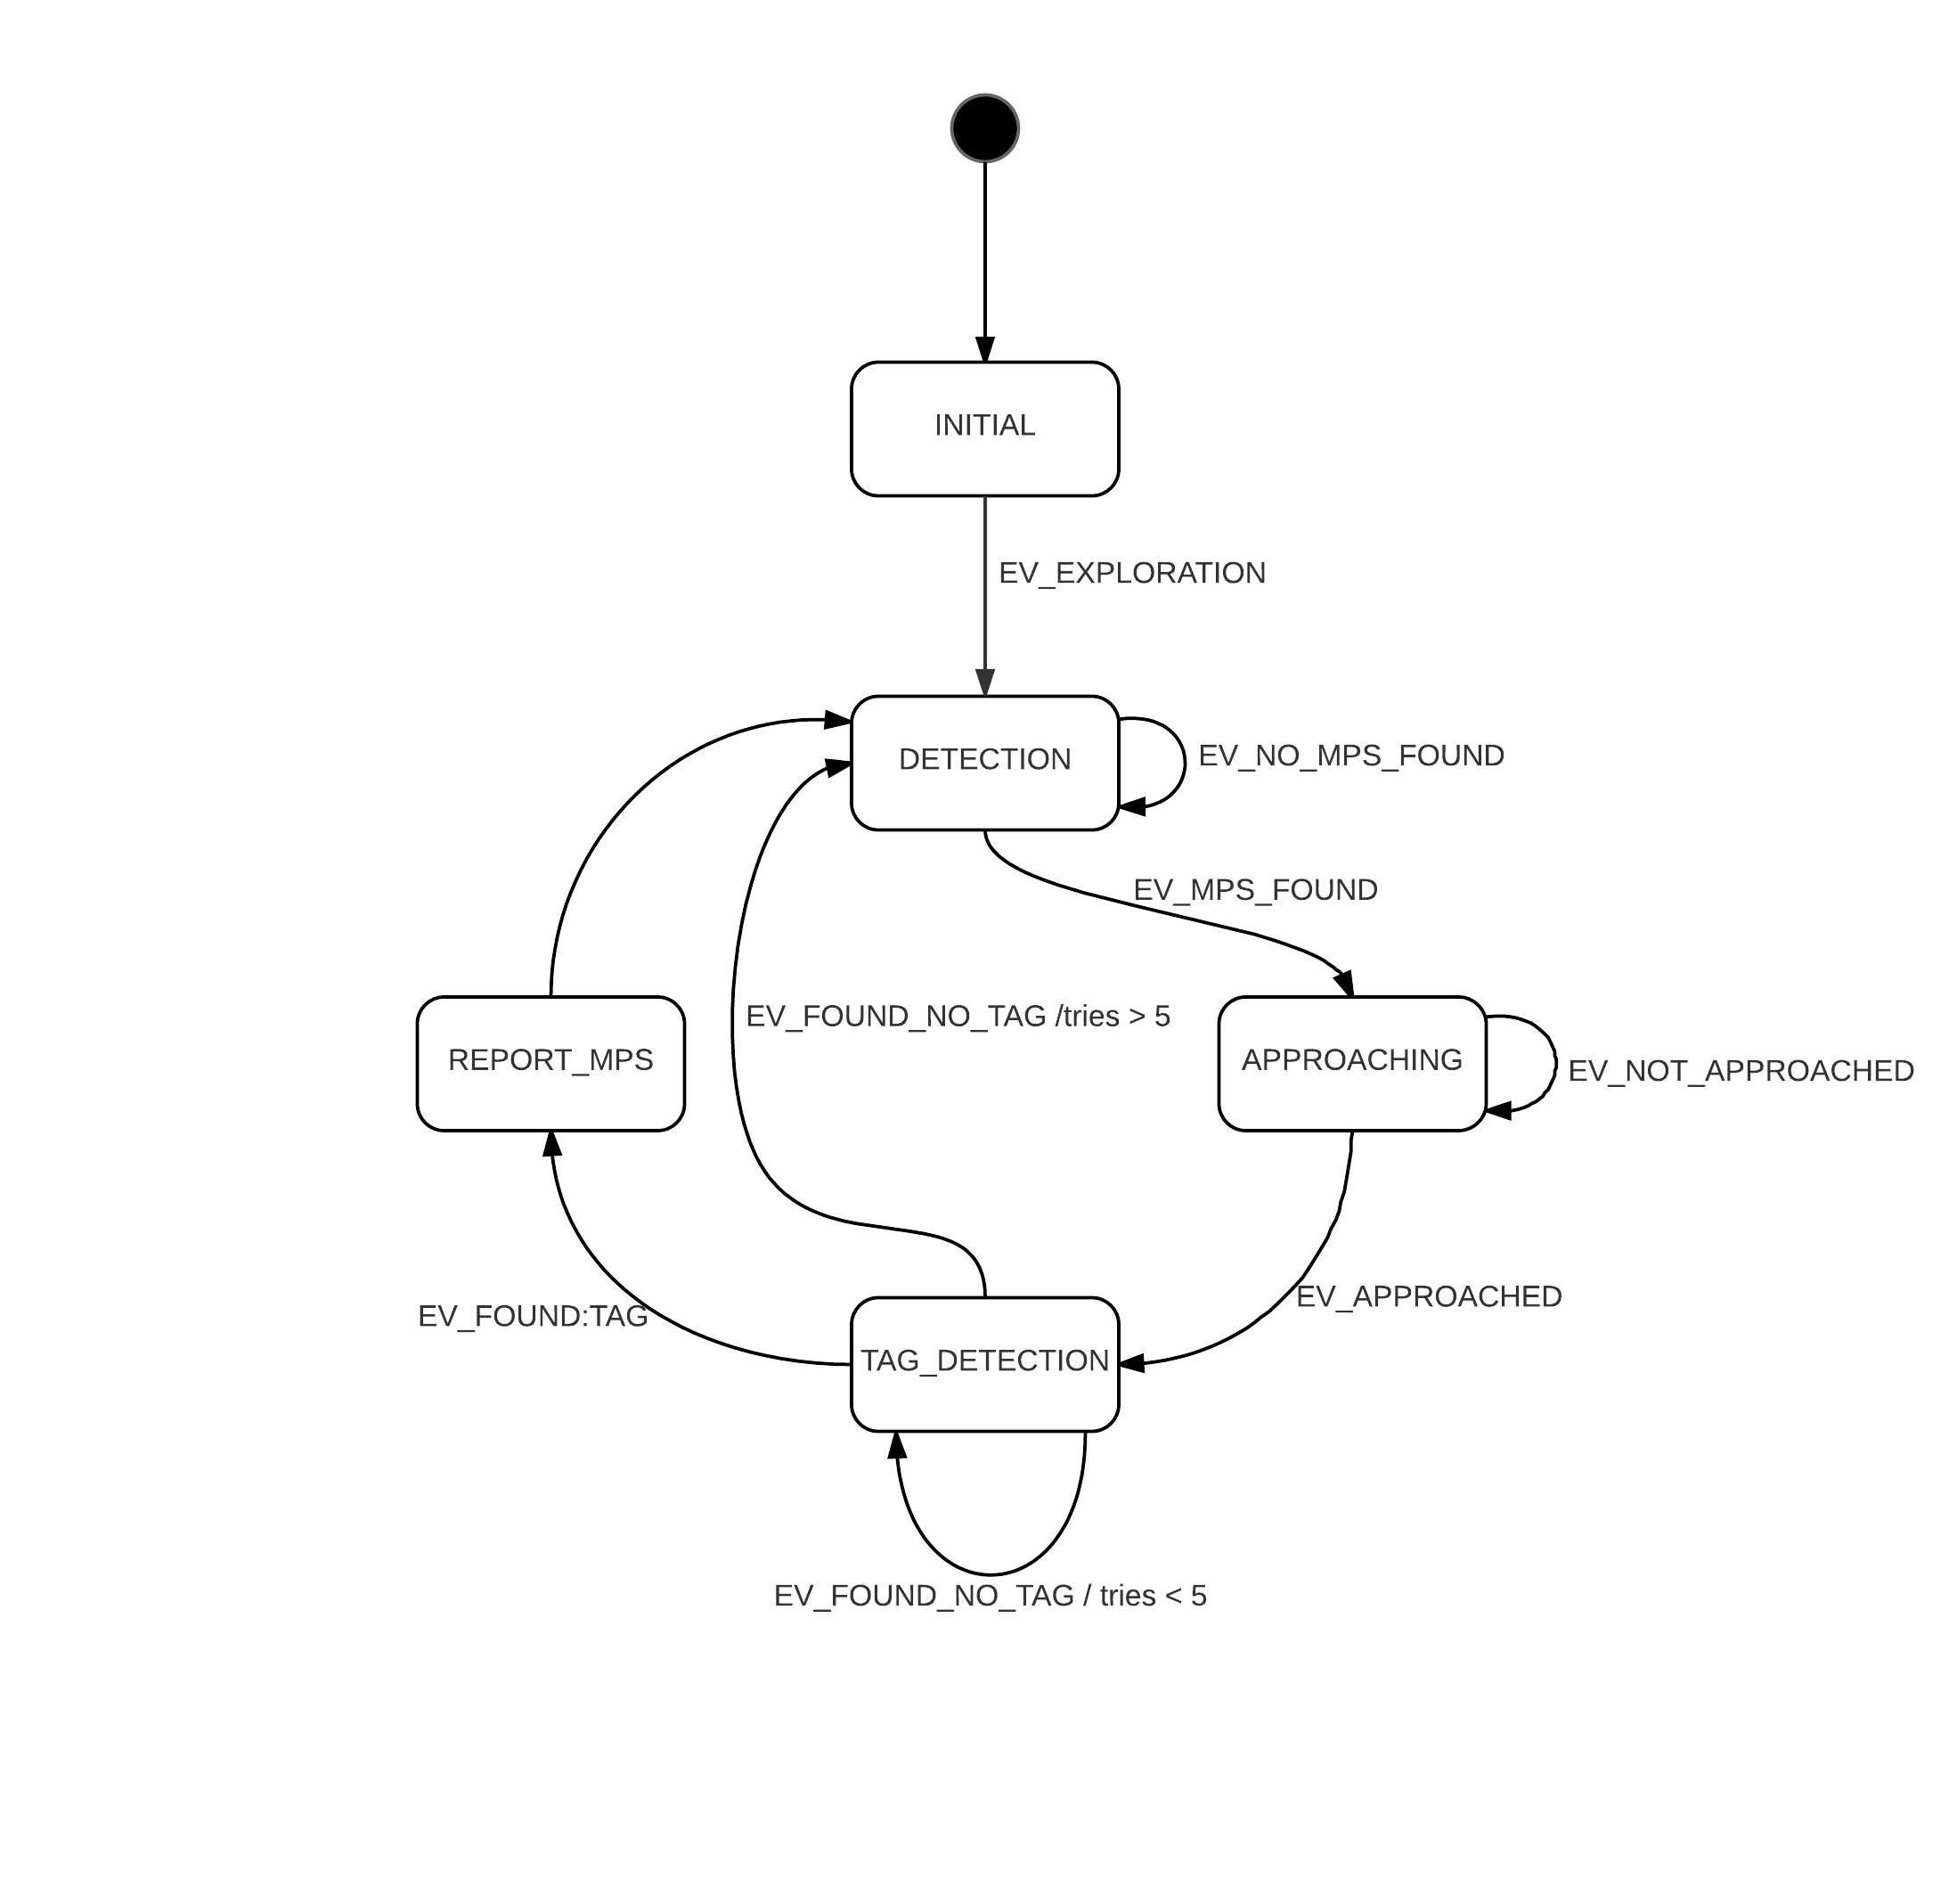
\includegraphics[scale=0.25]{pic/robotino_state_machine.png}
\caption{The statemachine for the exploration phase scenario}
\label{fig:statemachine}
\end{figure}

\newpage


The State machine contains the following states:

\begin{itemize}

\item INITIAL 

This is the first state the robot will transit into when launching up the robotino software for the Robocup competition. In this state the robot makes connection to the Referee Box and registers to the Referee system. After this it waits at the starting position for a signal which indicates that the exploration phase has begun. By receiving this message the robot makes a transition into the DETECTION state.  


\item DETECTION

In this state the robot drives around the field by following a line which is predefined by a set of landmarks on the field. While driving to a landmark the robot tries to detect MPS stations by using it's LIDAR ( Light Detection and Ranging cite here) sensor in the MPSDocking component. In this state the robot has two choices what to do next. As said before the transition between two states is triggered by a message which is received by the SmartRobotinoInstructionPlanner from one of the other components. In case of the DETECTION state this can be either if there was no MPS detected by the LIDAR sensor the MPSDocking component sends a message back which triggers the event EV\_NO\_MPS\_FOUND. Then the robot stays in the state and tries to detect more MPS stations while driving to the next landmark.  \\

If the MPSDocking component finds one or more MPS stations on the field this is transmitted to the Instruction Planner component. In this case a message is received with a list of all MPS stations, their docking points and the orientation is received. This triggers then a event with the name EV\_MPS\_FOUND. This event than induces a transition state to the APPROACHING state. 

\item APPROACHING 

This state is responsible for approaching a MPS station for a AlvarTagDetection or Docking operation. The robotino takes one of the MPS station which were detected in the previous state and drives in front of one of the docking points. Currently each MPS station has two docking points (one on the front and one on the back). To determine which docking point is the front or back, the AlvarTag needs to be scanned to find out the behavior of the MPS station. There are two outcomes in this state. If the goal (or the docking point) is not reached for now the robot stays in this state until the goal is reached. These actions are indicated by the events EV\_APPROACHED and EV\_NOT\_APPROACHED. Taking the first one of these two events can lead to a state transition into DETECTION state. This means that the robot is standing in front of the station and detection of the Alvartag can be started. 


\item TAG\_DETECTION

Detection of the AlvarTag fixed on the MPS station is done in the TAG\_DETECTION state. In this state the Instruction Planner sends a message to the AlvarTagDetection component to start the detection process. The AlvarTagDetection component than tries to detect the AlvarTag by taking pictures of the tag and runs an algorithm which can detect the information encoded in it. After the tag is detected from the AlvarTagDetection a message is send back to the Instruction Planner with the team color of the MPS station and the behavior of it (Ring Station, Cap Station and so on). Sometimes the tag is not detected correctly or it is an unknown tag the AlvarTagDetection sends back a message which triggers the EV\_FOUND\_NO\_TAG event. If this is the case the Instruction Planner retries the whole process for up to 5 times. If the tag is still not detected correctly after 5 times the Instruction Planner discards the tag detection and makes a transition into the DETECTION state. This is done due to the time constraints in the exploration phase. This is a sub-optimal solution because functionality like the quality of tag detection should not be a concern of the Instruction Planner but more the AlvarTagDetection. Therefore in the future this should be revised. \\

If the AlvarTag on the MPS station was detected correctly by the AlvarTagDetection component the Instruction Planner has now all the information which is needed to reply this to Referee Box. This is indicated by EV\_FOUND\_TAG event which leads to a state transition into the REPORT\_MPS state.


\item REPORT\_MPS

In this state the acquired information about the detected MPS stations is gathered together and send to the Referee Box. First the Instruction Planner converts the AlvarTag information from an internal representation into a representation which can be understood by the Referee Box. To archive this the information is packed into a communication object which is then send to the RefboxServer component which it then relays it to the actual Referee Box computer by using the Google Protobuff message protocol.  \\

After the information of the MPS station was transmitted to the Referee Box the Instruction Planner changes the state to the DETECTION state. Then the whole process is started again until the exploration phase is over. 


\end{itemize}


\subsubsection{Communication Objects Used in The Instruction Planner}


\begin{figure}[h]
\centering
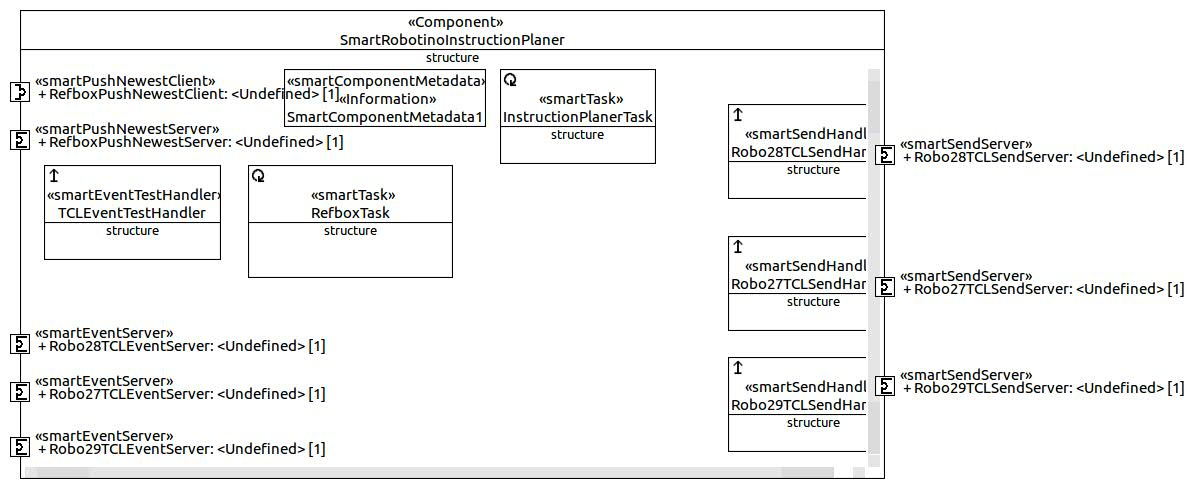
\includegraphics[scale=0.25]{pic/SmartRobotinoInstructionPlaner.JPG}
\caption{Model of Instruction Planner}
\label{fig:i_overview}
\end{figure}


As shown in figure \ref{fig:i_overview} the SmartRobotinoInstructionPlanner has multiple input and output ports which are connected to components such as RefboxServer, MPSDetection or AlvarDetection. This connection is created over the SmartLispServer component using SmartTCL messages. On the other hand connections to the SmartLogisticsRefboxServer are done over communication objects which can be created inside SmartSoft for data like the Phases, Maintenance and so on. For the connection between the Instruction Planner and the Refbox component a communication called CommRefbox is used. This object can be used to send certain data about the detected stations, exploration or production phase and the state of the robotino as seen by the 
Referee Box. \\

Currently the CommRefbox communication object can be used to transmit the following data: 

\begin{itemize}

\item MessageType

This describes the message type. This needs to be done because in C++ the type of an object (even if we have polymorphism) can be not be derived. Therefore each message needs a message type. Valid message types are: GAMESTATE, EXPLORATION\_INFO, MACHINE\_INFO, MACHINE\_REPORT, ORDER\_INFO and 
ROBOT\_INFO. 

\item Gamestate

The gamestate part of the communication object can be used to transmit the current gamestate from the RefBoxServer to the Instruction Planner. The elements of this sub-message is the state, phase and a time stamp. 

\item ExplorationInfo (deprecated)

This was originally intended to transmit a set of zones which can include a MPS station for the team with a high probability. But because of new rules in the 2017 scenario this was dismissed. Therefore this message part is currently out of use. The explorationInfo contains a array of probable zones. 


\item machineInfos

The machineInfos message contains a list of six machineInfo which can be used as database for already detected MPS stations. The list of machineInfo begins with mInfo1 and ends with mInfo6.

\item machineInfo

The machineInfo message describes the position of a detected MPS station with the X-Coordinate the Y-Coordinate and the orientation of the MPS-Station. This is exactly the data the Referee Box expects for a successful detection of the station.


\item machineReport


The machineReport describes general information about the detected MPS stations. The information which can be transmitted are the name of the MPS station, the zone where the MPS is localized, and the detected light signal. The lightsignal is deprecated in the 2017 scenario. 

\item robotInfo and robotState

These two message containers are used to transmit the current state of the robot as seen from the Refbox. The state of the robot can be ACTIVE if everything works normal, MAINTENANCE if the team asked for a maintenance break to fix some issue of the robot or DISQUALIFIED if the robot was put into maintenance the second time or violated some rule of the contest. This message is used for internal monitoring of the contest from the robot site. For example if the robot returns from reconnects to the Referee Box from a maintenance break it can detect whether it can start to drive into the field again.  


\item orderInfo

//todo 


\end{itemize}



\subsubsection{Advantages and Disadvantages of this design} 

\begin{itemize}

\item Advantages

For the design of the task instruction for the exploration phase, Event-driven finite-state machine was used. This pattern is often used in communication driven applications
like telecom software or communication protocols. Because the robotino software is distributed between a lot of components and these components need all to be coordinated and instructed a major component is needed which brings this all under the hood. Therefore a state machine is a good way to represent the exploration phase. The state machine is made out of states which represent certain logic blocks of the exploration phase. \\


Usually a logic block in the exploration phase is made out of a pattern:

\begin{enumerate}

\item Instruction Planner send a message to a component.

\item The component executes some task

\item The Instruction Planner receives a result if the task was executed successfully by the 
component or not.  


\end{enumerate}

For this pattern a message or event-driven state machine is really good match because the fact that a component like the AlvarTagdetection executes some logic can be designed as a state. For transition between several states the sending and receiving of messages can be used. For example to start a scan of the AlvarTag by the AlvarTagDetection component, a SmartTCL message needs to be send to the component. This induces a state transition into the state the AlvarTagDetection component is instructed to scan the tag. After the AlvarTagDetection component has finished with scanning it sends back a message which contains the tag of the MPS or a failure as the result. Using this message another state transition can be performed. \\

Because the exploration phase is made out of defined rules which the robot needs to be fulfill, this approach works well for this scenario. 


\item Disadvantages

A disadvantage is that the whole state machine needs to be handwritten by the developer because there is no tool included which can generate code out from a visual representation 
of the state machine. Although this is possible to use a separated tool, this is not included in smart soft. Therefore if a new logic block is added to the scenario by the rcll comitee this needs to be added by hand to the state machine. This can be a very time exhausting process if the state machine contains a lot of states. Therefore another design pattern might be better here which enables adding new logic blocks in a easier way. \\

Also another big disadvantage of this design is that functionality like this is already implemented inside the SmartSoft framework using the SmartTCL robotics behavior framework.
This framework enables it to model certain logic blocks of the exploration phase as robotic behaviors like "drive to a position" or "make a picture". The whole exploration phase can modeled using these SmartTCL task blocks. Writing these task blocks can be done using a DSL language which is implemented in Common Lisp. A disadvantage is that this Lisp based DSL is 
very different from general purpose languages like C++ or Java. But on the other side robotic tasks can be implemented easier. 


\end{itemize}


The current design is a hybrid out of SmartTCl and the event-driven finite state machine. The coordination between the components is done inside the C++ based RobotState class while the
triggering of the components is done via the Common Lisp based SmartLispServer. In the future this can be moved more to the SmartTCL implementation were the robot behavior is implemented in the SmartTCL DSL. 


\subsubsection{Maintenance Modes}

Describe how to team and the robot can react to failures and the system. How to set the robot into maintenance mode and how the robot can return to the game. 


\subsubsection{Outcome}

Multiple robots and Production phase







